\documentclass[english]{article}
\usepackage[T1]{fontenc}
\usepackage{natbib} % citations
\usepackage{csvsimple}
\usepackage{pgfplotstable}
\usepackage{rotating} % to rotate tables
%% tikz packages
\usepackage{tikz}
\usepackage{forest}
\usetikzlibrary{trees, arrows, shapes.geometric, positioning}
\usepackage{standalone}
%% text packages
\usepackage{siunitx} % fake ° symbol \ang{}
\usepackage[super]{nth} % for 1st, 2nd etc. \nth{}
\usepackage{hyperref}

\newcommand{\standartox}{STANDARTOX}
\newcommand{\epa}{EPA ECOTOX data base}
\newcommand{\rpackage}{http://139.14.20.252:3838/etox-base-shiny/}
\newcommand{\git}{https://github.com/andreasLD/etox-base}
\newcommand{\gitapp}{https://github.com/andreasLD/etox-base-shiny}
\newcommand{\ecfifty}{EC\textsubscript{50}}


\listfiles


\begin{document}


\title{Standartox: A tool to derive exposure endpoints from chemical test results}

\author{Andreas Scharm{\"u}ller\textsuperscript{1{*}},
        Verena Schreiner\textsuperscript{1},
        Ralf B. Sch{\"a}fer\textsuperscript{1}}

\maketitle
\thispagestyle{fancy}

1. Institute of Environmental Sciences, University of Koblenz-Landau Fortstraße 7, 76829 Landau, Germany {*}corresponding author(s):
Andreas Scharm{\"u}ller (andschar@protonmail.com)

\begin{abstract}
%%5This is a manuscript template for Data Descriptor submissions to \emph{Scientific
%%Data} (http://www.nature.com/scientificdata). The abstract must be
%%no longer than 170 words, and should succinctly describe the study,
%%the assay(s) performed, the resulting data, and the reuse potential,
%%but should not make any claims regarding new scientific findings.
%%No references are allowed in this section. 

<WRITE ABSTRACT>

\end{abstract}
\pagebreak

%%%%%%%%%%%%%%%%%%%%%% 01 Background

\section*{Background \& Summary [max 700 words]}

The risk of adverse effects of chemicals on the environment is globally assessed with the help of ecotoxicological tests that are conducted on different organism groups, ideally representing a specific biocoenosis and associated biotopes. These tests are conducted by different research groups all over the world who publish the results independently. Up to now, only few initiatives, such as the United States Environmental Protection Agency ECOTOXicology knowledgebase (EPA ECOTOX) \citep{elonen_ecotoxicology_2018}, the German Umweltbundesamt's Information System Ecotoxicology and Environmental Quality Targets (ETOX) \citep{umweltbundesamt_etox_2019} or the Pesticide Property Data Base (PPDB) aiming to consolidate ecotoxicological test results, exist. The former two collect test results and hence only partly check for quality whereas the latter aims for quality, yet being confined to specific classes of chemicals, in this case pesticides. An overall holistic approach in processing the large number of ecotoxicological test results is lacking. Therefore, we suggest Standartox, a tool and data base that aims to overcome these paucities by steadily incorporating the ever-growing number of test results in an automated process workflow that ultimately leads to single aggregated test results for specific chemical-organism test combinations, representing the toxicity of a chemical. Automated approaches are increasingly important because a growing number of chemicals such as pharmaceuticals, pesticides and synthetic hormones, amongst others are in daily use all over the world with insufficient knowledge about possible adverse effects on the environment. Generally, chemicals are brought to the environment deliberately - as it is the case of pesticides, or arrive therein as a byproduct from other processes (e.g. atmospheric emissions or wastewater) \citep{schwarzenbach_challenge_2006}. In turn, ecosystems provide essential services to human societies such as drinking and irrigation water, food and climate regulation. These services are products of different ecosystem functions that crucially depend on the integrity of the populations and communities that drive these ecosystem functions. However, besides habitat degradation, climate change and nutrient enrichment, pollution with man-made chemicals threatens these populations and communities in various ways which are currently not fully understood \citep{steffen_anthropocene_2007}. Pollution with man-made chemicals was indeed identified as one of three major environmental problems for which research gaps hamper the derivation of planetary boundaries, i.e. thresholds beyond which irreversible state shifts may occur \citep{steffen_anthropocene_2007}. Bernhardt et al. \citet{bernhardt_synthetic_2017} argue further that the knowledge gap how chemicals effect populations and communities and hence ecosystem functions and ecosystem services, would also impede society's ability to accomplish the Sustainable Development Goals of the United Nations. In Europe alone some 100,000 chemicals are estimated to be in current use, whereof 30,000 are produced in quantities larger than one ton per year \citep{breithaupt_costs_2006}. Data on toxicity tests for a lot of chemicals, especially newly emerging ones remains scarce and if existent, the information is represented sparsely and in inconsistent formats \citep{gessner_fostering_2016}. Therefore, tools such as Standartox are a required step adding a layer of abstraction satisfying the needs of modern environmental risk assessment demands. Standartox aggregates ecotoxicological test results in a standardized and reproducible way, providing the basis for the derivation of risk indicators such as Species Sensitivity Distributions (SSD) \citep{posthuma_species_2002} and Toxic Units (TU), which represent two prominent concepts to assess effects on organisms in ecotoxicology \citep{kefford_definition_2011, schafer_effects_2011}. Besides aggregating ecotoxicological test results, Standartox provides a concise overview of the status of tested chemicals, allowing the identification of potential research gaps. Standartox comes with two front-ends, an R \citep{rcoreteam_language_2017} package and a web tool, adding convenience structures and largely reducing work time for users.

%%%%%%%%%%%%%%%%%%%%%%%%%%%%%%%%%%%%%%%%%% IDEAS %%%%%%%%%%%%%%%%%%%%%%%%%%%%%%%%%%%%%%%%%
\iffalse



Curently \citep{schafer_future_2019} 

include \citep{yamamuro_neonicotinoids_2019} and \citep{seibold_arthropod_2019} as a new prominent examples for effects on the ecosystem


    \item standardized toxicity values
    
    \item reproducible
    
    \item time saving
\fi    

%%%%%%%%%%%%%%%%%%%%%%%%%%%%%%%%%%%%%%%%%% OLD %%%%%%%%%%%%%%%%%%%%%%%%%%%%%%%%%%%%%%%%%%%
\iffalse

A large number of chemicals such as pharmaceuticals, pesticides and synthetic hormones are in daily use all over the world with insufficient knowledge about possible adverse effects on the environment. In Europe alone some 100,000 chemicals are estimated to be in current use, whereof 30,000 are produced in quantities larger than one ton per year \citep{breithaupt_costs_2006}. Chemicals are brought to the environment deliberately - as it is the case of pesticides, or arrive therein as a byproduct from other processes (e.g. atmospheric emissions or wastewater) \citep{schwarzenbach_challenge_2006}. Ecosystems provide essential services to human societies such as drinking and irrigation water, food and climate regulation. These services are products of different ecosystem functions that crucially depend on the integrity of the populations and communities that drive these ecosystem functions. However, besides habitat degradation, climate change and nutrient enrichment, pollution with man-made chemical toxicants threatens these populations and communities in various ways which are currently not fully understood \citep{steffen_anthropocene_2007}. Pollution with man-made chemical toxicants was indeed identified as one of three major environmental problems for which research gaps hamper the derivation of planetary boundaries, i.e. thresholds beyond which irreversible state shifts may occur \citep{steffen_anthropocene_2007}. Bernhardt et al. \citet{bernhardt_synthetic_2017} argue further that the knowledge gap how chemicals effect populations and communities and hence ecosystem functions and ecosystem services, would also impede society's ability to accomplish the Sustainable Development Goals of the United Nations. According to Breithaupt \citet{breithaupt_costs_2006} less than one percent of chemicals released to the environment are thoroughly tested. Although for some chemicals advanced and standardized \citep{oecd_oecd_2018} test methods have been developed, ecotoxicological tests for a lot of chemicals, especially newly emerging ones remain scarce and if existent, the information is represented sparsely and in inconsistent formats. \citep{gessner_fostering_2016}. Therefore we developed a data base that collects, processes and aggregates ecotoxicological tests results in order to subsequently publish it in an harmonized form as a web application - the \etoxbase{} tool: \href{http://139.14.20.252:3838/etox-base-shiny/}. This should facilitate researchers the access to ecotoxicological test results and support modern chemical risk assessment (CRA) workflows. The \etoxbase{} makes use of ecotoxicological test data, obtained from the ECOTOXicology knowledgebase (ECOTOX) created by the U.S. Environmental Protection Agency (EPA). ECOTOX collects raw, non harmonized ecotoxicological test data on aquatic and terrestrial wildlife as well as plants and publishes it on a quarterly basis. By the time of writing it contained 926,108 test results, comprising 11,685 chemicals tested on 12,668 different species \citep{elonen_ecotoxicology_2018}. The collected ecotoxicological test data contain a variety of measured endpoints such as Effective Concentrations (\ecfifty{}) values, No-observed effect concentrations (NOEC) or lowest observed effect concentrations (LOEC). Likewise the data set contains different effect measures such as mortality, intoxication and growth as well as a multiplicity of test durations ranging from seconds to weeks or even years. The \etoxbase{} aggregates this information according to the user's inputs. These can then be used for the derivation of risk indicators such as Species Sensitivity Distributions (SSDs) \citep{posthuma_species_2002} and Toxic Units (TUs), which represent two prominent concepts to assess effects on organisms in ecotoxicology. The former combines toxicity data of several organism groups towards a chemicals to estimate effects on biotic communities, the latter refers to effects of a specific organism (group) towards a chemical. The two concepts are widely used in ecotoxicology \citep{kefford_definition_2011, schafer_effects_2011} since the allow for a comparison of toxicities across multiple chemicals and biological communities, respectively. Although performed on one and the same organism and chemical, outcomes of different ecotoxicological tests vary greatly due to differences in test parameters, genetic differences in individual populations or other irrepressible factors making a selection of appropriate test results for CRA laborious. The \etoxbase{} aims to relief this process and provide single toxicity values for organism, chemical and test duration combinations. The \etoxbase{} downloads every new version of the ECOTOX data base and performs several quality checks, e.g. unit harmonization, and cleaning steps on it. Hence, new scientific test results are constantly incorporated. Additionally the \etoxbase{} queries chemical- and organism-specific variables from other open data bases to fill information gaps such as water solubility, organism habitat or regional occurrence patterns in the ECOTOX data base.

\fi


\pagebreak

%%%%%%%%%%%%%%%%%%%%%% 02 Methods

\section*{Methods}

%%The Methods should include detailed text describing any steps or procedures 
%%used in producing the data, including full descriptions of the experimental 
%%design, data acquisition assays, and any computational processing (e.g. 
%%normalization, image feature extraction). Related methods should be grouped 
%%under corresponding subheadings where possible, and methods should be described 
%%in enough detail to allow other researchers to interpret and repeat, if required, 
%%the full study. Specific data outputs should be explicitly referenced via data 
%%citation (see Data Records and Data Citations, below). Authors should cite 
%%previous descriptions of the methods under use, but ideally the method 
%%descriptions should be complete enough for others to understand and reproduce 
%%the methods and processing steps without referring to associated publications. 
%%There is no limit to the length of the Methods section.

The \etoxbase{} consists of two parts of software: Firstly a processing pipeline (Fig. \ref{fig:pipeline}) downloads quarterly released new versions of the \epa{} and performs several preparation steps in R \citep{r_core_team_r_2017}, to then store the outcome in a PostgreSQL data base. This constitutes the basis upon which the R shiny web application is accessing the data \citep{r_core_team_r_2017}. The application itself is set of R functions that filter and aggregate the data according to a user's inputs \ref{fig:app}. Finally in the web application, a `filtered` and an `aggregated` data set as well as an interactive plot, for data exploration are returned. These two data sets can be downloaded. In the following these two parts are explained in detail, naming the respective R scripts in brackets.

\subsection*{Data acquisition \& preparation}

(bd\_epa\_download.R) 
(bd\_epa\_postgres.R)
(da\_epa1.R, da\_epa2.R, da\_epa3.R)
(qu\_aw.R)
(qu\_chemspieder\_scrape.R) 
(qu\_pc.R) 
(qu\_pp.R)
(qu\_worms2.R) 
(qu\_rgbif.R) 
(re\_merge.R) 
(re\_combine.R)
(re\_checks\_internal.R) 
(re\_analyses.R)
(re\_final.R)

The EPA ECOTOX data is downloaded and subsequently built into a PostgreSQL data base. Afterwards the data is imported into R for pre-processing, which includes validity checks, removal of special characters, unit harmonizations and selection of relevant variables. Chemical abstract service (CAS) numbers, unique chemical identifiers together we taxon names are then used to query other data bases for additional information on chemicals and biota respectively. Chemical information is retrieved from the Compendium of Pesticide Common Names \citep{CITE_AW}, the Chemspider data base \citep{CITE-CHEMSPIDER}, from Eurostat <CITATION>, the Pubchem data base \citep{CITE_PUBCHEM}, and from the Physprop data base \citep{CITE_PHYSPROP}. These queries mostly rely on the webchem R-package \citep{szocs_webchem_2015-1}. For biota, habitat and occurrence information is queried from the World Register of Marine Species (WORMS) \citep{WORMS} and from the Global Biodiversity Information Facility (GBIF) \citep{CITE_RGBIF} using the rgbif R-package \citep{chamberlain_rgbif_2018}. The acquired information is then merged and information is combined. From there on the data set is analyzed and checked and finally compiled in one table. This table is then used as the input for the filter and aggregation functions \ref{fig:pipeline}. For a detailed overview of what information is collected see table \ref{tab:scripts-pipeline}.

\begin{figure}
    \includestandalone[width=\textwidth, scale=0.1]{tikz/pipeline_organigram}
    \caption{Processing Pipeline}
    \label{fig:pipeline}
\end{figure}


\subsection*{The application}
The application is accessible through \app{} and was built in R, using the shiny web application framework \citep{chang_shiny_2018}. Users can define several input parameters \ref{tab:inputs} in the application's graphical user interface (GUI), handled in the ui.R script in order to adjust the aggregation according specific requirements. In doing so users execute R functions (fun\_filter.R, fun\_aggregation.R, fun\_filagg\_plot\_ly.R) loaded in the server.R script, which produce a 'filtered' and an 'aggregated' data set as well as an interactive overview plot. Only the 'aggregated' data set is presented in the GUI. However, both data sets can be downloaded via a download button.

\begin{figure}
    \includestandalone[scale=0.75]{tikz/application}
    \caption{Application}
    \label{fig:app}
\end{figure}

\subsection*{Aggregation}
The \etoxbase{} application aggregates the test results according to chosen filters in a two step process. Firstly the filtered test results are aggregated by the CAS number, the chosen taxon and the selected test duration. Secondly, the returned data is then aggregated by the CAS number. The former can't be influenced by the user and calculates either the minimum or the median depending on the amount of results to aggregate (n <= 2: minimum, if n > 2: median). Thereof the second step calculates the minimum, the maximum, the median, the geometric mean, or the arithmetic mean as an aggregate. 

\subsection*{Code availability}
%%For all studies using custom code in the generation or processing of datasets, 
%%a statement must be included here, indicating whether and how the code can be 
%%accessed, including any restrictions to access. This section should also include 
%%information on the versions of any software used, if relevant, and any specific 
%%variables or parameters used to generate, test, or process the current dataset. 

The processing code is stored in a Github reopsitory (\git{}). All processing scripts were written in R version 3.4.4. PostgreSQL 9.5 has been used to build the data base. Hence, R together with its packages \ref{tab:rpackages} and PostgreSQL suffice to rebuild the process. The code of the application itself is stored in a second Github repostitory (\gitapp{}). Since new versions of the EPA ECOTOX data base are published on a quarterly basis the data acquisition process is automated and new versions of the application are scheduled to be released regularly.

\begin{table}[h!]
    \centering
    \begin{tabular}{|l|l|l|l|}
        \hline
        Category        & Package       & Version   & Reference                     \\ \hline
        processing      & RCurl         & 1.95-4.11 & \citep{lang_rcurl_2018}       \\ \hline
        processing      & data.table    & 1.12.0    & \citep{dowle_data.table_2018} \\ \hline
        application     & shiny         & 1.1.0     & \citep{chang_shiny_2018}      \\ \hline
    \end{tabular}
    \caption{List of R packages used in compiling the data.\newline{}
    TODO: Automate version input and name generation - whole table\newline{}
    TODO2: debug chang\_shiny\_2018 reference}
    \label{tab:rpackages}
\end{table}


\section{TODO}

    \item it is planed to extend this tool to other data bases if they provide new test data  (e.g. UBA ETOC)
\pagebreak

%%%%%%%%%%%%%%%%%%%%%% 03 Data records
%%Please explain each data record associated with this work, including
%%the repository where this information is stored, and an overview of
%%the data files and their formats. Each external data record should
%%be listed in Data Citation section at the end of this template, and 
%%records should be cited throughout the manuscript as, for example 
%%(Data Citation 1). 
%%
%%Tables should be used to support the data records, and should clearly indicate 
%%the samples and subjects, their provenance, and the experimental manipulations 
%%performed on each. They should also specify the data output resulting from each 
%%data-collection or analytical step, should these form part of the archived record. 
%%Please see the submission guidelines at the \emph{Scientific Data} website, and 
%%our Word templates for more information on preparing such tables. 


\section*{Data Records}

Explain the data




\pagebreak

%%%%%%%%%%%%%%%%%%%%%% 04 Technical validation
%%This section presents any experiments or analyses that are needed
%%to support the technical quality of the dataset. This section may
%%be supported by up figures and tables, as needed. This is a required
%%section; authors must present information justifying the reliability
%%of their data.
\section{Technical validation}

\subsection{Unit Harmonisation}
In order to guarantee appropriate conversion and harmonisation of units we take a random sample of the 50 most occurring concentration units (Table \ref{tab:chck-concentration}) as well as six of the most occurring duration units (Table \ref{tab:chck-duration}) and convert them manually to subsequently compare them to the conversions done by Standartox. This is check is done whenever Standartox is rebuilt.

\subsection{Comparison to other data bases}
In order to asses the validity of the Standartox approach to aggregate test results we compared Standartox values with effect values for the same chemicals and the same test duration from the PPDB (n=3601) \ref{fig:standartox_ppdb_diff}. This showed that 91.3\% of the Standartox values diverge by less than a factor of 10 from the PPDB values. Considering only Standartox values for which at least five of ten tests were aggregated the value increases to 91.7\% and 93.4\% respectively. Admittedly a few Standartox values diverge by a large margin.

\begin{figure}
    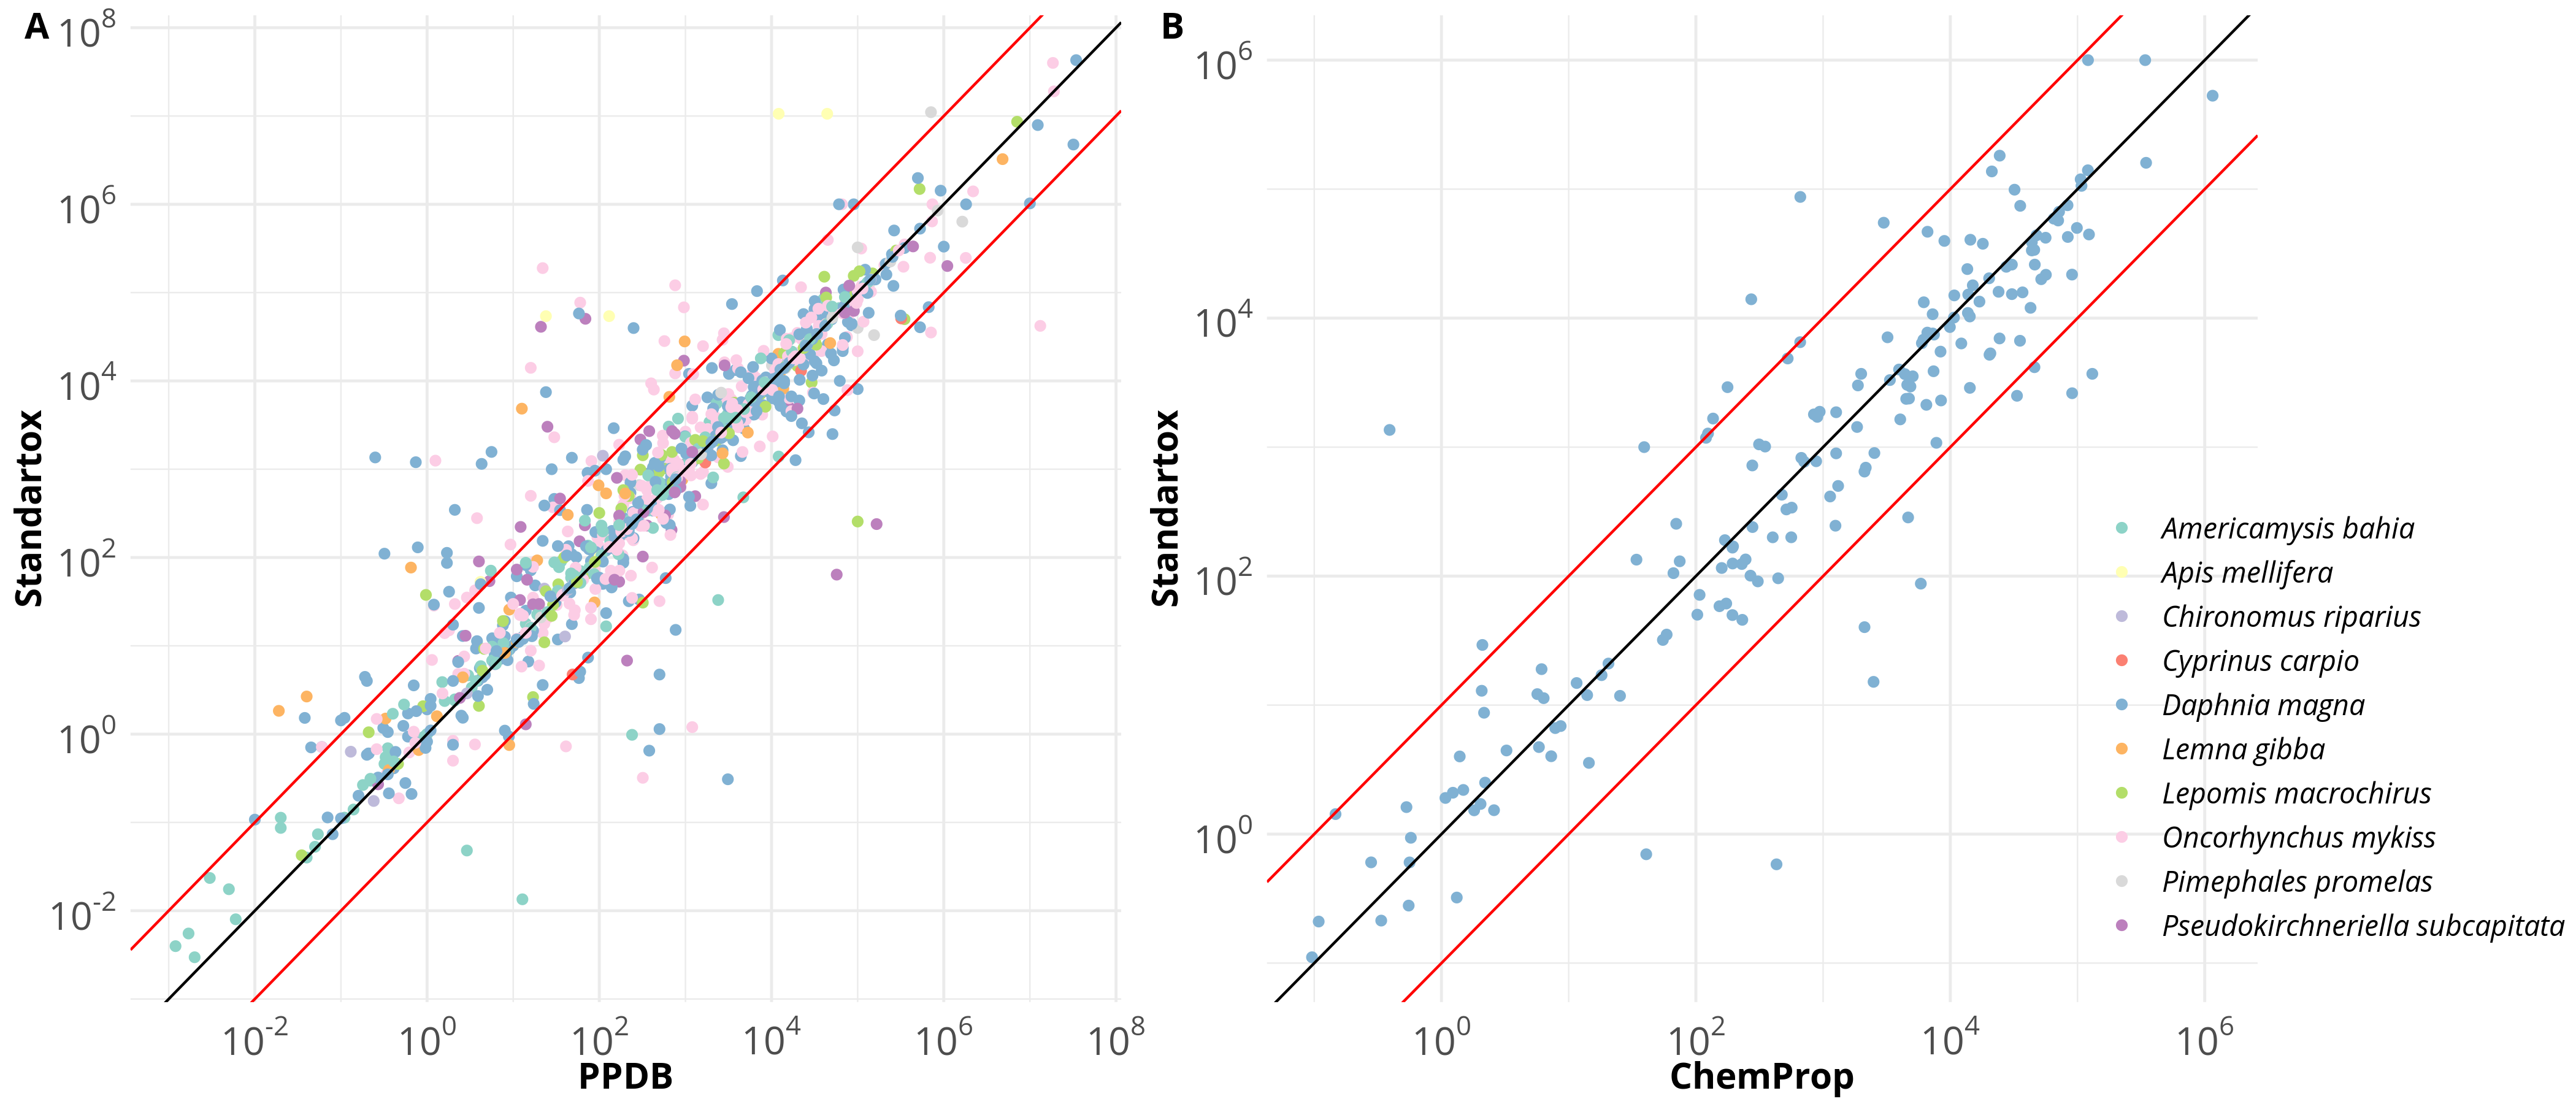
\includegraphics[width=1\linewidth]{article/figures/gg_ppdb_stan_compare_continous.png}
    \caption{Comparison between Standartox and PPDB values}
    \label{fig:standartox_ppdb_diff}
\end{figure}

\subsection{Overall distribution of tests}
Heatmap: don't Include for now. Too large.
Put maybe a plotly on wep app
Mybe search for the 50 most sold chemicals and asses the number of tests


In order to validate Standartox we compared resulting values with values from other data bases, such as the PPDB. Of 542 chemicals, only 16\% diverged from the PPDB values by a factor greater than 10, supporting plausibility of the \standartox results \ref{fig:standartox_ppdb_diff}.



\pagebreak

%%%%%%%%%%%%%%%%%%%%%% 05 Usage notes
\section*{Usage Notes}
%%Brief instructions that may help other researchers reuse these dataset.
%%This is an optional section, but strongly encouraged when helpful
%%to readers. This may include discussion of software packages that
%%are suitable for analyzing the assay data files, suggested downstream
%%processing steps (e.g. normalization, etc.), or tips for integrating
%%or comparing this with other datasets. If needed, authors are encouraged
%%to provide code, programs, or data processing workflows when they may help 
%%others analyse the data. We encourage authors to archive related code in 
%%a DOI-issuing archive when possible, but code may also be supplied as 
%%supplementary information files. 
%%
%%For studies involving privacy or safety controls on public access
%%to the data, this section should describe in detail these controls,
%%including how authors can apply to access the data, and what criteria
%%will be used to determine who may access the data, and any limitations
%%on data use.
Standartox can either be accessed through the APP or the API together with the R-package standartox. Both access pathways allow for the same filters and aggregation methods (Table \ref{tab:app-parameters} to be applied on the data. In the former the user can download the resulting data sets as a comma-separated values file whereas in the latter the user can directly load them in R. The user can choose among different parameters to filter and aggregate the test data accordingly \ref{tab:app-parameters}. The user can filter for compound-specific filters, including the CAS number, the concentration type (e.g. Active Ingredient, Formulation), the chemical class (e.g. Insecticides, Metals) and taxon-specific filters, including common taxonomic groups (e.g. Daphniidae, Algae), the habitat (e.g. freshwater) and the regional occurrence (e.g. Europe, Asia) of the organisms. Furthermore, the user can refine the results to specific test durations (in hours), effect groups (e.g. Mortaliy, Population, Growth) and endpoints (EC\textsubscript{50}, EC\textsubscript{10}, LOEC or NOEC).  As aggregates the user can choose the minimum, the maximum, the median, the geometric mean or the arithmetic mean. All the steps described in this section are selectable in the GUI and are executed at each click by the application. The drop down menu `Download data` allows to download a filtered data set as well as an aggregated data set.

Percentage values next to inputs show the proportion of the respective option (e.g. \textit{Active Ingredient - 43\%} indicates that 43\% of the data are Active Ingredients).

\subsection*{R package}
The R-package standartox consists of the two functions stx\_catalog() and stx\_query(). The former allows the retrieval of a catalog of possible parameters that can be used as an input for the latter. stx\_query() fetches the toxicity values from the data base and returns them as a R list object (compare Code \ref{listing:standartox-example}).

\begin{lstlisting}[
    caption = {standartox R-package code} example,
    label = {listing:standartox-example}]
# install
install.packages('remotes')
remotes::install_github('andschar/standartox') # package not yet on CRAN
# retrieve catalog    
require(standartox)
catal = stx_catalog()
# retrieve data
l = stx_query(cas = '1071-83-6',
                endpoint = 'XX50',
                taxa = 'Oncorhynchus',
                duration = c(24, 120))
\end{lstlisting}

Standartox is designed to support CRA. With an increased amount of available ecotoxicological test data, it becomes fundamental to provide and distribute such information in reasonable formats, meaning accessible for humans as well as machines. Currently CRA often relies on test results of a few, well tested standard organism, such as \textit{Daphnia magna}, \textit{Pimephales promelas}, \textit{Selenastrum capricornutum}, although researchers have conducted experiments on a much greater variety of organisms (e.g. the 926,108 test results collected in the EPA ECOTOX data base). In order to locate ecotoxicological test data, researchers can rely on individual test results reported in publications <CITE>, on compiled and published data sets \citep{malaj_organic_2014} or on data bases such as the Pesticide Property Data Base (PPDB) \citep{lewis_international_2016}. Each data source has its limitations though: Collecting toxicity information from individual publications is laborious and using already compiled data from publications or data bases is often limited to a specific groups of chemicals, such as pesticides, biozides etc. Standartox, making use of the EPA ECOTOX, the largest publicly available collection of ecotoxicological test results, aims to facilitate the data retrieval process by providing adequate aggregates (EC\textsubscript{50}, NOEC, LOEC) of the tests results. These are then used for the calculation of SSDs, TUs or other risk indicators. SSDs try to extrapolate effects of chemicals towards organisms from species to a community level by fitting a statistical distribution to toxicity test results on organisms of different trophic levels in order to derive concentrations at which a specific fraction of organisms are effected (often at 5\% - HC\textsubscript{5} \citep{posthuma_species_2002}. Figure \ref{fig:ssd-isoproturon} shows an example of a SSD and the derived HC\textsubscript{5} value (red dassed line) created for the herbicide Isoproturon. TUs are another indicator of effects of chemicals on organisms. They are calculated by dividing a measured concentration (c) by an EC\textsubscript{50} value (cf. Equation \ref{eq:tu}).

\begin{equation}
    TU_i = \frac{c_i}{\ecfifty}
    \label{eq:tu}
\end{equation}

\begin{figure}[h!]
    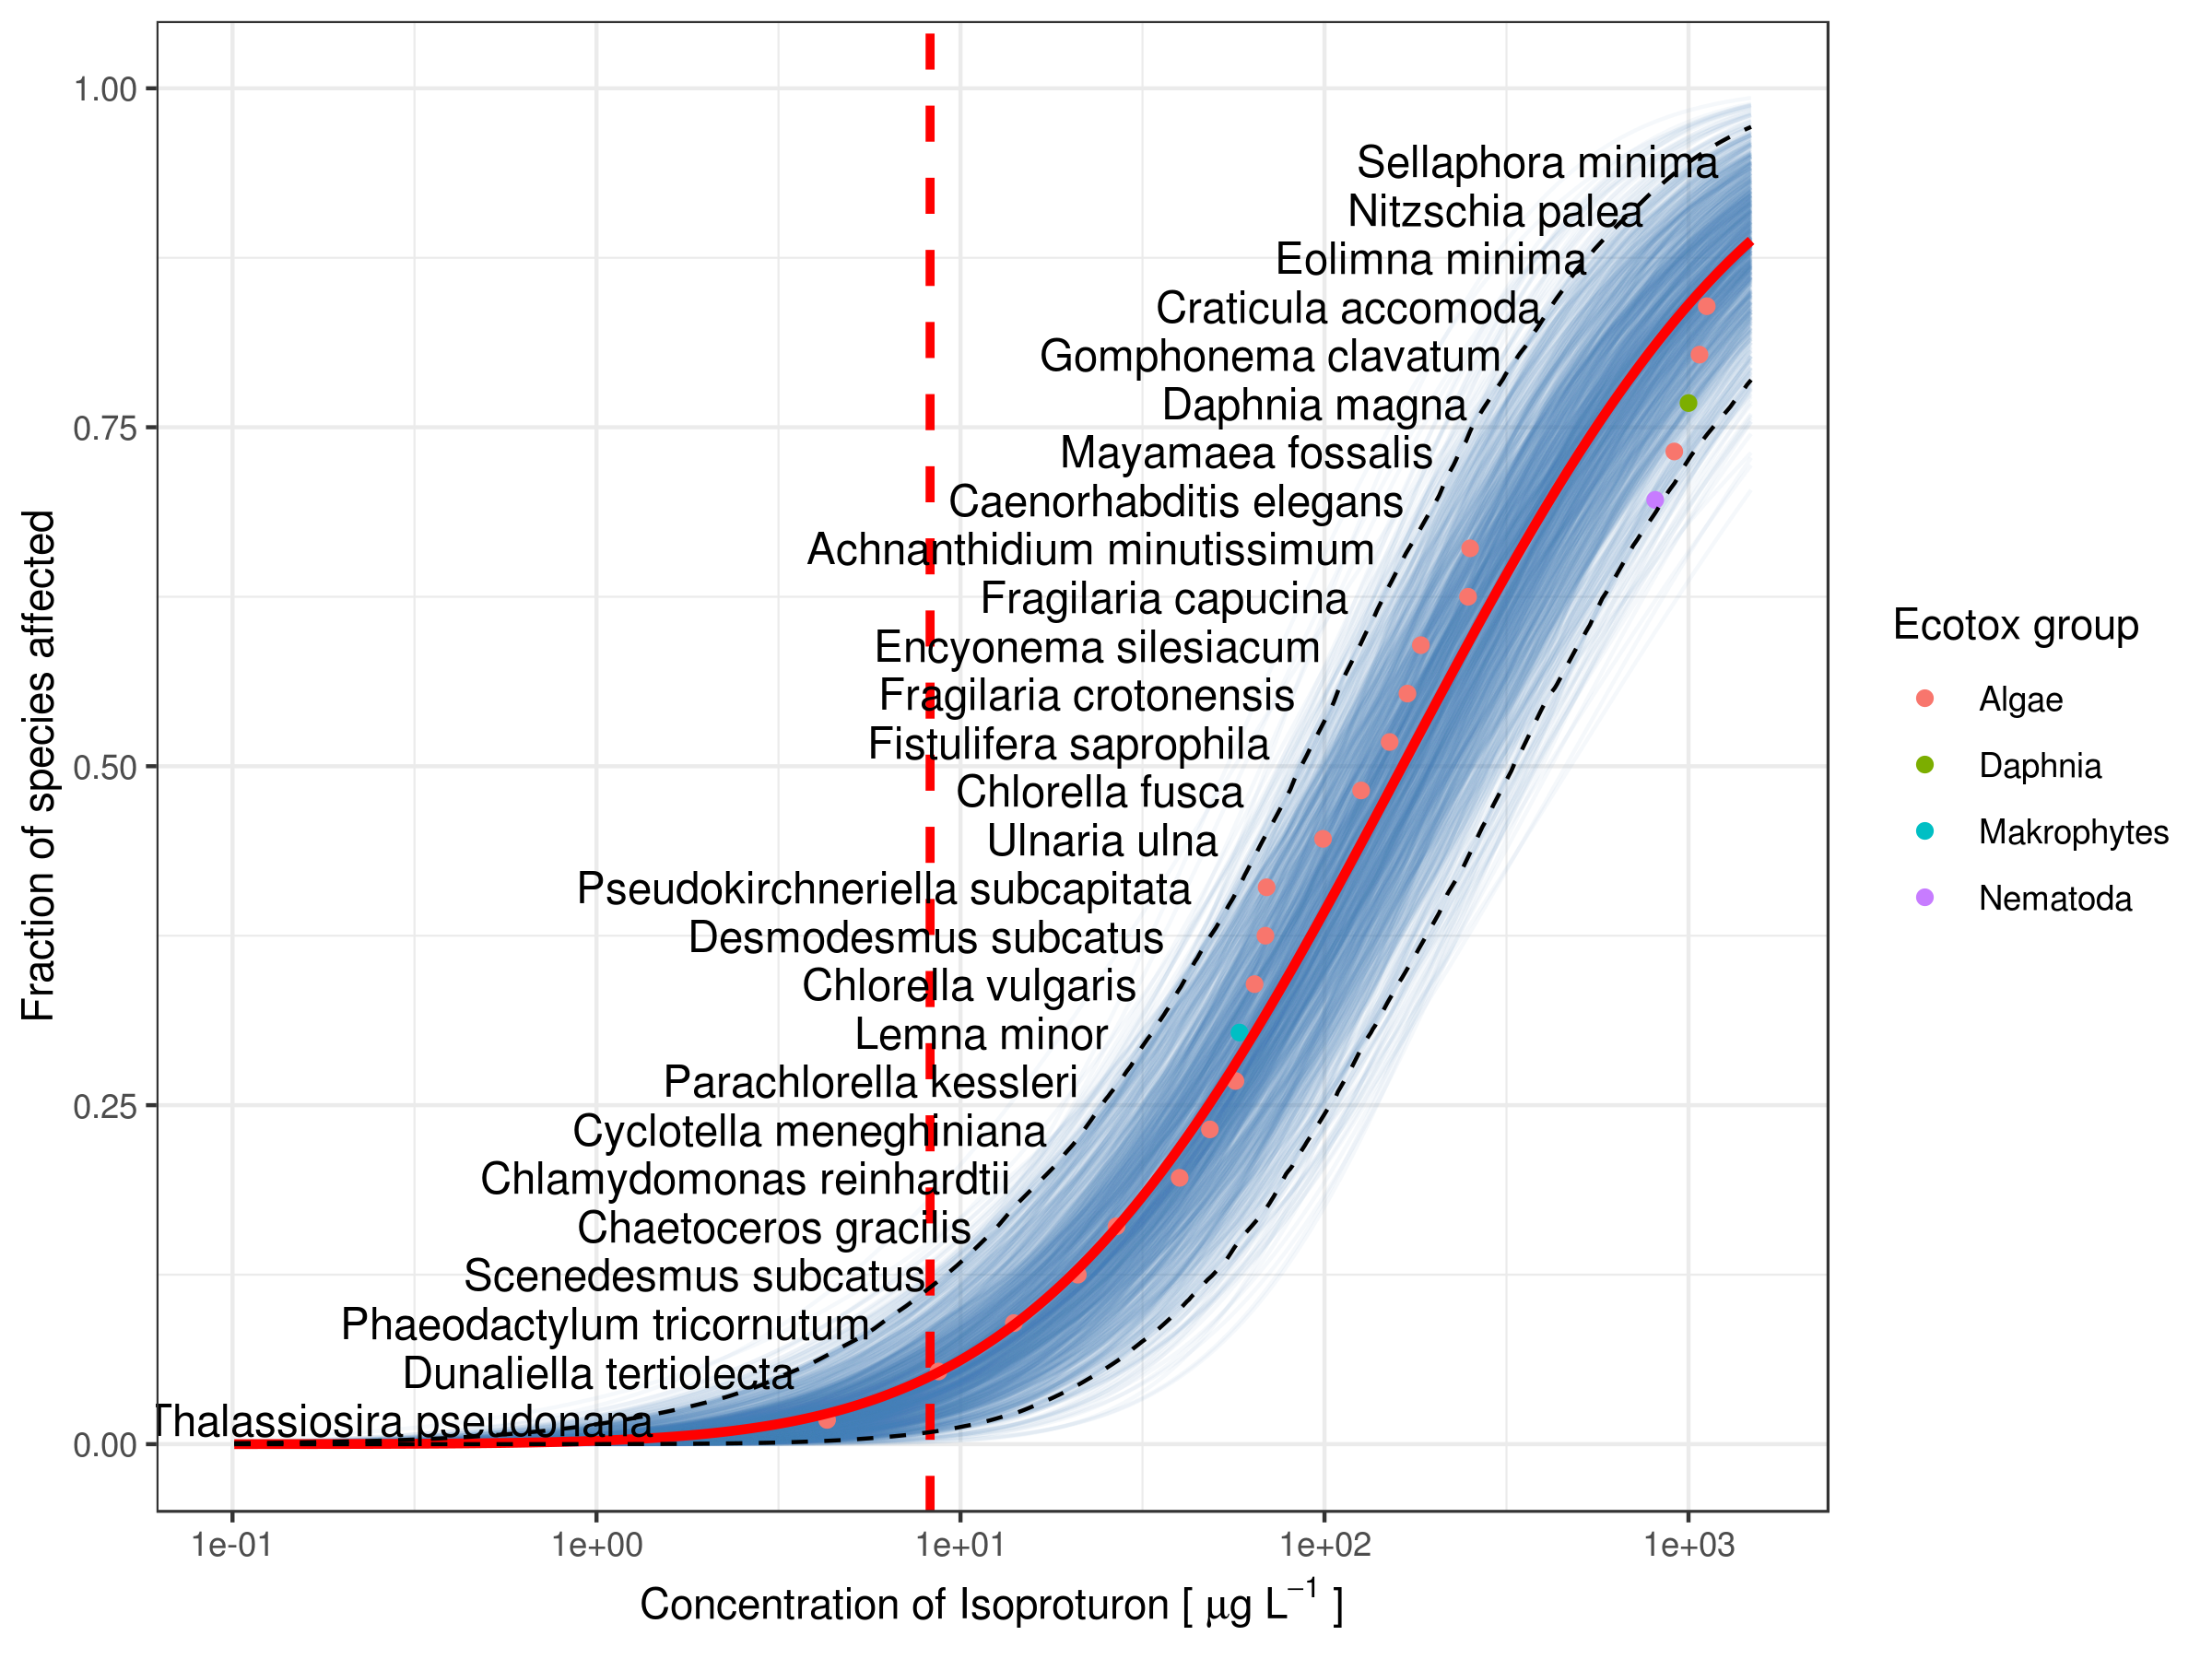
\includegraphics[width=1\linewidth]{article/figures/ssd2_boot.png}
    \caption{SSD plot showing the susceptibility of organisms towards the herbicide Isoproturon. The red line represents the fit and the red dashed line marks the HC\textsubscript{5} value, which is a common measure in CRA. The legend denotes common organism groups used in ecotoxicology.}
    \label{fig:ssd-isoproturon}
\end{figure}


\subsection*{Limitations}
Since the EPA ECOTOX data at hand merely represents a sample of the reality of the toxicity of chemicals on organisms, it has to be stated that the returned Standartox values are subject to change. New studies will be published and constantly incorporated into Standartox, improving the toxicity estimates. However, we expect values of well tested chemical-organism combinations to be relatively stable. A future analysis on the smallest number of tests needed to return trustworthy results, could shed more light on this aspect. Furthermore, toxicity test results are certainly influenced by individual tests parameters, such as pH, temperature or conductivity amongst others \citep{rosenkrantz_influence_2013, li_temperature_2011}. Such information is not included in the aggregation performed by Standartox, since the EPA ECOTOX only provides sparse records on those. Most frequently provided test parameters (and their percentage) are medium temperature (77\%), pH:56\%, hardness:27\%, dissolved oxygen:18\%, Alkalinity:15\% and salinity:9\%. Others are provided for less than 5\% of the tests. A test-mining approach, iterating through the individual test studies could potentially increase this number. However, we argue that using the geometric mean as an aggregate allows for an adequate estimation of the toxicity of a chemical towards an organism group. We prefer the geometric mean in comparison to the arithmetic mean, since it is considerably less influenced by outliers and is suitable for skewed data. Also, the geometric mean is preferable over the median, since the median completely ignores the influence of large or small values, making it unreliable for small data sets <CITATION GEOMETRIC MEAN>.

\subsection*{Other data bases}
Other initiatives tidying the large number of ecotoxicological test results were also developed recently. They partly aim for overlapping goals, yet have limitations or objectives that differentiate them from Standartox. Since 2006, the PPDB provides validated ecotoxicological information on pesticides \citep{lewis_international_2016}.
% TODO lookup NORMAN citation
The Network of reference laboratories, research centres and related organisations for monitoring of emerging environmental substances (NORMAN) focuses on assembling river basin specific pollutants \citep{von_der_ohe_new_2011}. 
Connors et al. \citet{healthandenvironmentalsciencesinstitutehesi_envirotox_2019, connors_creation_2019} published the EnviroTox data base \href{https://envirotoxdatabase.org/} which also uses, amongst others the EPA ECOTOX data as an input. In comparison to Standartox, ENviroTox focuses only on aquatic organisms and uses an qualitative algorithm to exclude unreliable test results. They filter for example the data to fish, amphibian invertebrate and algae taxa, to test durations of above 24 hours and aquatic taxa only and add additional information on toxicity endpoints, such as chronic or acute tests as well as mode of action assignments. In contrast, Standartox doesn't refine to specific test durations, but leaves it up to the user to decide on such parameters. The EnvirTox data base also allows for an aggregation of test results to derive single toxicity values for individual taxa whereas Standartox performs this aggregation for individual chemicals. This has to be done in a cumbersome way by down- and uploading the data manually. Comptox, is a web tool published by the EPA which, similar to Standartox allows for filtering test results and the retrieval of additional chemical information. However, it lacks the possibility to aggregate toxicity test results \citep{usenvironmentalprotectionagency_comptox_2019}. Petschick et al. (in submission) modeled risk threshold level equivalents for aquatic organisms by using ecotoxicological effect data from the EPA ECOTOX. However, none of the above mentioned approaches aim for a standardized aggregation method of toxicity endpoints for individual chemicals. Besides, they also lack the possibility for automated and scriptable user requests for high level programming languages, such as R or Python. Along with newly created ecotoxicological data bases here, methods of how to efficiently store ecotoxicological data are also proposed as can be seen in the MAGIC Knowledge Base \citep{bub_graphing_2019}. This recent increase of efforts to compile ecotoxicological test data bases clearly emphasizes the need for holistic and automated analyses of large-scale ecotoxicological data. Standartox is a tool that puts its focus on the aggregation of toxicity data and by this adds a piece to the puzzle of modern ecotoxicological analyses.

\subsection*{Identify chemicals to be tested}
There is a clear need in ecotoxicology for harmonised approaches to collect ecotoxicological data as other data base compilation attempts recently published show. Hitchock et al. \citet{hitchcock_improving_2018} argue for an increased awareness concerning newly published ecotoxicological test results to facilitate meta analyses across studies. Important statistical parameters, such as mean estimates, variances and sample sizes. Likewise, state variables, including medium temperature, pH, mineral contents or organism age and sex should be reported (if not in the text, in an online repository). Standartox doesn't include such information mainly because the EPA ECOTOX reports only a few of these variables. A future research aim could be to use machine learning techniques to retrieve this information from the referenced articles.
Above all, recent studies showed that, in defiance of many regulation efforts \citep{schafer_future_2019} chemicals can still cause strong adverse effects on organisms and in turn the environment. Neonicotinoids, a group of insecticides was for example related to declines in insectivorous birds \citep{hallmann_declines_2014} and fish yields due to cascading food web effects \citep{yamamuro_neonicotinoids_2019}. Standartox provides means to synthesise ecotoxicological test data, thereby identify research gaps. Furthermore, standardized approaches could potentially reduce unnecessary animal testing by synthesizing existing ecotoxicological test data.

\begin{figure}
    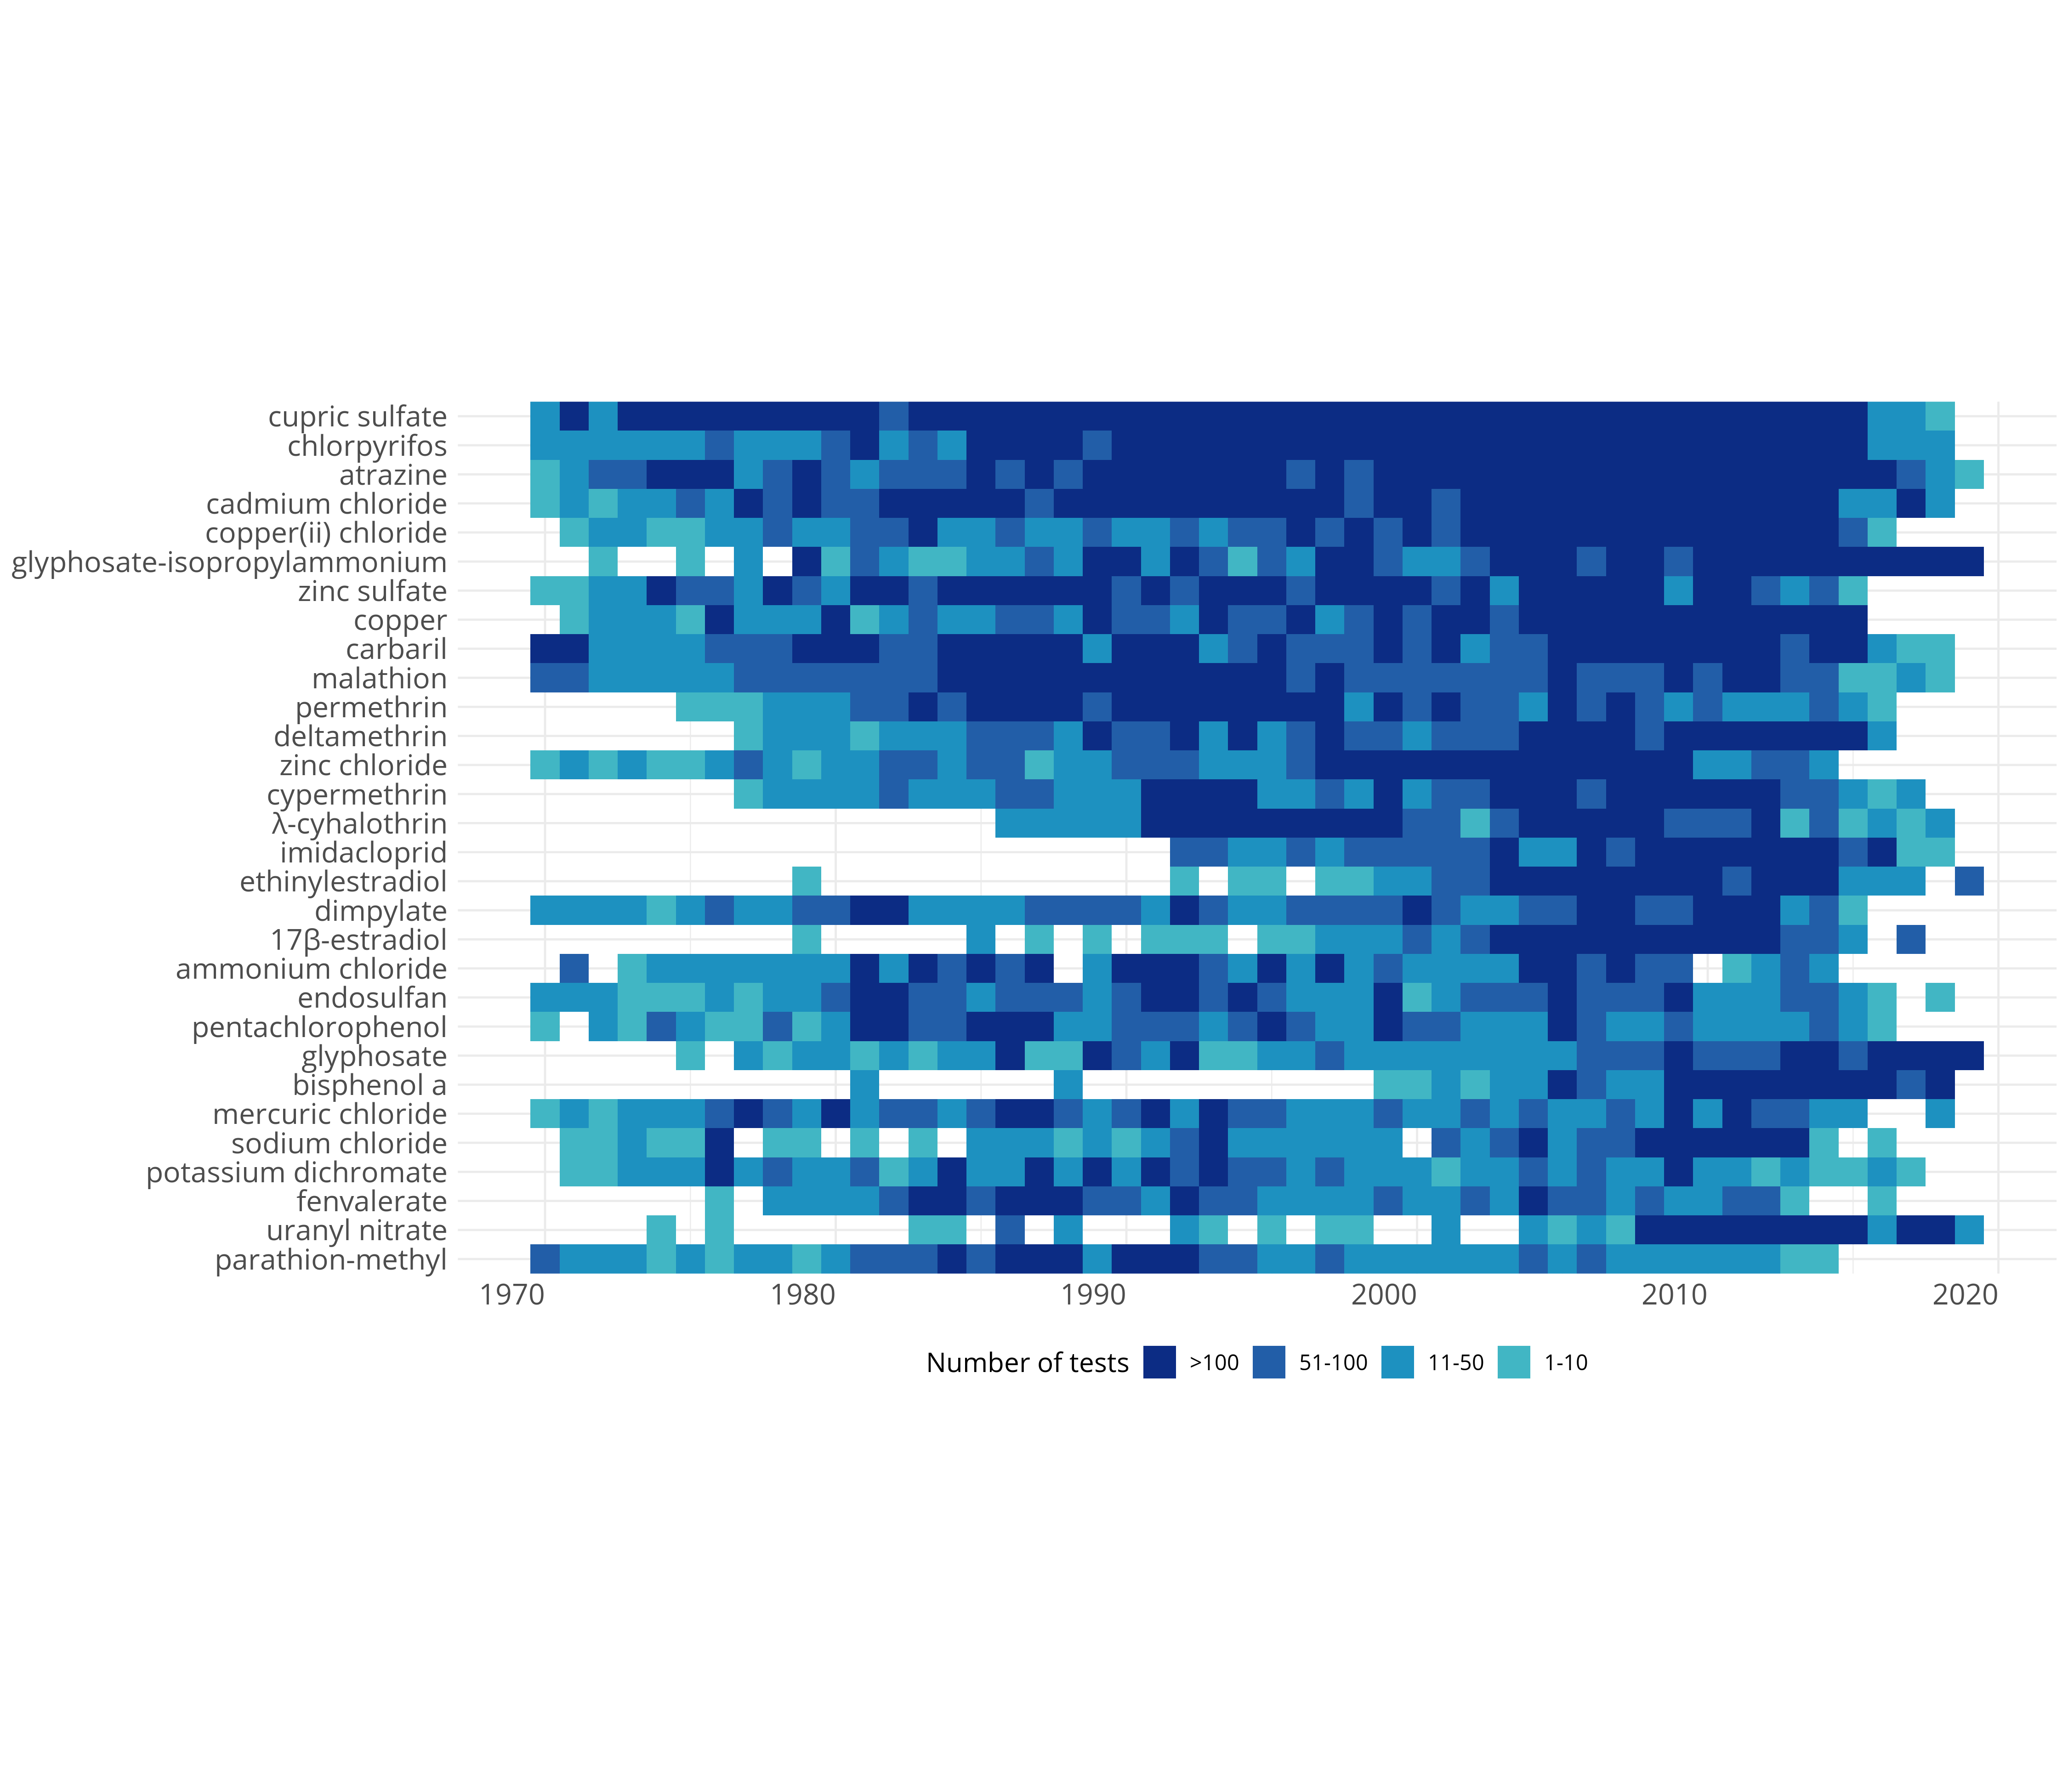
\includegraphics[width=1\linewidth]{article/figures/heatmap_tests_n.png}
    \caption{30 most tested chemicals in EPA ECOTOX.}
    \label{fig:standartox_ppdb_diff}
\end{figure}

%%%%%%%%%%%%%%%%%%%%%%%%%%%%%%%%%%%%%%%%%% TODO %%%%%%%%%%%%%%%%%%%%%%%%%%%%%%%%%%%%%%%%%%
1) \citep{staveley_challenge_2016} describe what is necessary for future ecotoxicology.

%%%%%%%%%%%%%%%%%%%%%%%%%%%%%%%%%%%%%%%%%% OLD %%%%%%%%%%%%%%%%%%%%%%%%%%%%%%%%%%%%%%%%%%%
\iffalse
Besides that, two cleaning steps can also be chosen. Firstly the application allows to exclude test results exhibiting concentrations that are higher than the actual water solubility of the respective chemical at \ang{20} C. Secondly the user can choose to exclude outliers (cf. Table \ref{tab:scripts-app}). The outliers are selected as values that exceed lower (0.25) and the upper (0.75) quartile by 1.5 times the inter-quartile range.
\fi


\section*{Acknowledgements}
%%Text acknowledging non-author contributors. Acknowledgements should
%%be brief, and should not include thanks to anonymous referees and
%%editors, or effusive comments. Grant or contribution numbers may be
%%acknowledged. Author contributions Please describe briefly the contributions
%%of each author to this work on a separate line. 
%%
%%AK did this and that. 
%%
%%BG did this and that and the other. 


\section*{Competing financial interests}
%%A competing financial interests statement is required for all accepted
%%papers published in \emph{Scientific Data}. If none exist simply write,
%%``The author(s) declare no competing financial interests''.


\section*{Figures Legends}
%%Figure should be referred to using a consistent numbering scheme through
%%the entire Data Descriptor. For initial submissions, authors may choose
%%to supply this document as a single PDF with embedded figures, but
%%separate figure image files must be provided for revisions and accepted
%%manuscripts. In most cases, a Data Descriptor should not contain more
%%than three figures, but more may be allowed when needed. We discourage
%%the inclusion of figures in the Supplementary Information \textendash{}
%%all key figures should be included here in the main Figure section. 
%%
%%Figure legends begin with a brief title sentence for the whole figure
%%and continue with a short description of what is shown in each panel,
%%as well as explaining any symbols used. Legend must total no more
%%than 350 words, and may contain literature references. 


\section*{Tables}
%%Tables supporting the Data Descriptor. These can provide summary information
%%(sample numbers, demographics, etc.), but they should generally not
%%be used to present primary data (i.e. measurements). Tables containing
%%primary data should be submitted to an appropriate data repository. 
%%
%%Tables may be provided within the \LaTeX{} document or as separate
%%files (tab-delimited text or Excel files). Legends, where needed,
%%should be included here. Generally, a Data Descriptor should have
%%fewer than ten Tables, but more may be allowed when needed. Tables
%%may be of any size, but only Tables which fit onto a single printed
%%page will be included in the PDF version of the article (up to a maximum
%%of three). 

%\begin{sidewaystable}
%    \csvautotabular[respect all]{data/meta.csv};
%    \caption{Meta variables table};
%    \label{table:meta-variables};
%\end{sidewaystable}




\pagebreak

\bibliographystyle{apalike}
\bibliography{refs/references-standartox.bib} % only reference from Zotero to avoid key conflicts
% NOTE multiple refs would have to be written w/o space and separated by <,>

\section*{Data Citations}

\pagebreak
\section*{TODO}

\begin{itemize}

\item compare Etox-BAse output with PPDB

\item plot example SSD and TU

\item acute vs chronic

\item OECD guidlines are not machine readable

\item discuss flaws in column types (e.g some concentration entries contain '+' or '~' and are therefore not convertable to numeric) - This hampers large scale analysis greatly!

\pagebreak
\section*{MISC}

\begin{figure}
    \includestandalone[scale=0.5]{tikz/tree_source}
    \caption{Alternative processing pipeline}
    \label{fig:pipeline-tree}
\end{figure}

\section*{not included citations}

\item Put in citation \citep{hartung_chemical_2009} ? which claims that REACH won't meet their assumptions and say 54 million vertebrate animals are needed for tests that would cost €9.5 billion over the next ten years. I.e 20 times more animals, 6 times the costs in comparison to the official estimates 

\item "comparison of rate of change in the production and variety of pesticides, pharmaceuticals and other chemicals over the past four decades to CO2 nutrient pollution and other global change factors" \citep{bernhardt_synthetic_2017}

\item worldwide decline in entomofauna: \citep{sanchez-bayo_worldwide_2019}


\end{itemize}

\pagebreak
\section*{Supplement}
\subsection*{R-package list} %% TODO put in appropriate list
Rinker TW, Kurkiewicz D (2018).
\emph{pacman: Package Management for R}.
version 0.5.0, \url{http://github.com/trinker/pacman}.
\newline R Core Team (2019).
\emph{R: A Language and Environment for Statistical Computing}.
R Foundation for Statistical Computing, Vienna, Austria.
\url{https://www.R-project.org/}.
\newline Wickham H, Hester J, Chang W (2019).
\emph{devtools: Tools to Make Developing R Packages Easier}.
R package version 2.2.1, \url{https://CRAN.R-project.org/package=devtools}.
\newline Lang DT, team tC (2019).
\emph{RCurl: General Network (HTTP/FTP/...) Client Interface for R}.
R package version 1.95-4.12, \url{https://CRAN.R-project.org/package=RCurl}.
\newline Wickham H (2019).
\emph{stringr: Simple, Consistent Wrappers for Common String Operations}.
R package version 1.4.0, \url{https://CRAN.R-project.org/package=stringr}.
\newline Bengtsson H (2019).
\emph{R.utils: Various Programming Utilities}.
R package version 2.9.0, \url{https://CRAN.R-project.org/package=R.utils}.
\newline Hiebert J (2016).
\emph{udunits2: Udunits-2 Bindings for R}.
R package version 0.13, \url{https://CRAN.R-project.org/package=udunits2}.
\newline Wickham H (2019).
\emph{rvest: Easily Harvest (Scrape) Web Pages}.
R package version 0.3.4, \url{https://CRAN.R-project.org/package=rvest}.
\newline Wickham H (2019).
\emph{httr: Tools for Working with URLs and HTTP}.
R package version 1.4.1, \url{https://CRAN.R-project.org/package=httr}.
\newline Ooms J (2014).
``The jsonlite Package: A Practical and Consistent Mapping Between JSON Data and R Objects.''
\emph{arXiv:1403.2805 [stat.CO]}.
\url{https://arxiv.org/abs/1403.2805}.
\newline Wickham H, Bryan J (2019).
\emph{readxl: Read Excel Files}.
R package version 1.3.1, \url{https://CRAN.R-project.org/package=readxl}.
\newline Walker A (2019).
\emph{openxlsx: Read, Write and Edit XLSX Files}.
R package version 4.1.0.1, \url{https://CRAN.R-project.org/package=openxlsx}.
\newline Henry L, Wickham H (2019).
\emph{purrr: Functional Programming Tools}.
R package version 0.3.2, \url{https://CRAN.R-project.org/package=purrr}.
\newline Dowle M, Srinivasan A (2019).
\emph{data.table: Extension of `data.frame`}.
R package version 1.12.4, \url{https://CRAN.R-project.org/package=data.table}.
\newline Conway J, Eddelbuettel D, Nishiyama T, Prayaga SK, Tiffin N (2017).
\emph{RPostgreSQL: R Interface to the 'PostgreSQL' Database System}.
R package version 0.6-2, \url{https://CRAN.R-project.org/package=RPostgreSQL}.
\newline R Special Interest Group on Databases (R-SIG-DB), Wickham H, Müller K (2018).
\emph{DBI: R Database Interface}.
R package version 1.0.0, \url{https://CRAN.R-project.org/package=DBI}.
\newline Oksanen J, Blanchet FG, Friendly M, Kindt R, Legendre P, McGlinn D, Minchin PR, O'Hara RB, Simpson GL, Solymos P, Stevens MHH, Szoecs E, Wagner H (2019).
\emph{vegan: Community Ecology Package}.
R package version 2.5-5, \url{https://CRAN.R-project.org/package=vegan}.
\newline Wickham H (2011).
``The Split-Apply-Combine Strategy for Data Analysis.''
\emph{Journal of Statistical Software}, \bold{40}(1), 1--29.
\url{http://www.jstatsoft.org/v40/i01/}.
\newline Komsta L (2011).
\emph{outliers: Tests for outliers}.
R package version 0.14, \url{https://CRAN.R-project.org/package=outliers}.
\newline Wickham H (2019).
\emph{feather: R Bindings to the Feather 'API'}.
R package version 0.3.3, \url{https://CRAN.R-project.org/package=feather}.
\newline Wickham H (2016).
\emph{ggplot2: Elegant Graphics for Data Analysis}.
Springer-Verlag New York.
ISBN 978-3-319-24277-4, \url{https://ggplot2.tidyverse.org}.
\newline Slowikowski K (2019).
\emph{ggrepel: Automatically Position Non-Overlapping Text Labels with
'ggplot2'}.
R package version 0.8.1, \url{https://CRAN.R-project.org/package=ggrepel}.
\newline Wilke C (2019).
\emph{cowplot: Streamlined Plot Theme and Plot Annotations for 'ggplot2'}.
R package version 0.9.4, \url{https://CRAN.R-project.org/package=cowplot}.
\newline Neuwirth E (2014).
\emph{RColorBrewer: ColorBrewer Palettes}.
R package version 1.1-2, \url{https://CRAN.R-project.org/package=RColorBrewer}.
\newline Tennekes M (2017).
\emph{treemap: Treemap Visualization}.
R package version 2.4-2, \url{https://CRAN.R-project.org/package=treemap}.
\newline Chamberlain S, Barve V, Mcglinn D, Oldoni D, Desmet P, Geffert L, Ram K (2019).
\emph{rgbif: Interface to the Global Biodiversity Information Facility API}.
R package version 1.3.0, \url{https://CRAN.R-project.org/package=rgbif}.

Chamberlain S, Boettiger C (2017).
``R Python, and Ruby clients for GBIF species occurrence data.''
\emph{PeerJ PrePrints}.
\url{https://doi.org/10.7287/peerj.preprints.3304v1}.
\newline Scott Chamberlain, Eduard Szocs (2013).
``taxize - taxonomic search and retrieval in R.''
\emph{F1000Research}.
\url{http://f1000research.com/articles/2-191/v2}.

Chamberlain S, Szoecs E, Foster Z, Arendsee Z, Boettiger C, Ram K, Bartomeus I, Baumgartner J, O'Donnell J, Oksanen J, Tzovaras BG, Marchand P, Tran V, Salmon M, Li G, Grenié M (2019).
\emph{taxize: Taxonomic information from around the web}.
R package version 0.9.7, \url{https://github.com/ropensci/taxize}.
\newline Arel-Bundock V, Enevoldsen N, Yetman C (2018).
``countrycode: An R package to convert country names and country codes.''
\emph{Journal of Open Source Software}, \bold{3}(28), 848.
\url{https://doi.org/10.21105/joss.00848}.
\newline Microsoft, Weston S (2017).
\emph{foreach: Provides Foreach Looping Construct for R}.
R package version 1.4.4, \url{https://CRAN.R-project.org/package=foreach}.
\newline Corporation M, Weston S (2018).
\emph{doParallel: Foreach Parallel Adaptor for the 'parallel' Package}.
R package version 1.0.14, \url{https://CRAN.R-project.org/package=doParallel}.
\newline Klik M (2019).
\emph{fst: Lightning Fast Serialization of Data Frames for R}.
R package version 0.9.0, \url{https://CRAN.R-project.org/package=fst}.
\newline Xie Y, Cheng J, Tan X (2019).
\emph{DT: A Wrapper of the JavaScript Library 'DataTables'}.
R package version 0.7, \url{https://CRAN.R-project.org/package=DT}.
\newline Tennekes M (2017).
\emph{treemap: Treemap Visualization}.
R package version 2.4-2, \url{https://CRAN.R-project.org/package=treemap}.
\newline 
\pagebreak

\subsection*{Data base tables}
\begin{table}[ht]
  \caption{Table of queried data bases}
  \label{tab:data-base}
  \centering
\begin{tabular}{ll}
  \hline
  Data Base & URL \\ 
  \hline
  Chemical Entities of Biological Interest (ChEBI) & https://www.ebi.ac.uk/chebi \\ 
  Chemical Identifier Resolver & https://cactus.nci.nih.gov/chemical/structure \\
  ChemSpider & http://www.chemspider.com \\
  Eurostat & https://ec.europa.eu/eurostat/home \\
  PHYSPROP Database & https://www.srcinc.com/what-we-do/environmental/scientific-databases.html \\
  PubChem & https://pubchem.ncbi.nlm.nih.gov \\ 
  Wikidata & https://www.wikidata.org/wiki/Wikidata:Main_Page \\
  Global Biodiversity Information Facility (GBIF) & https://www.gbif.org \\
  World Register of Marine Species (WoRMS) & http://marinespecies.org \\
  \hline
\end{tabular}
\end{table}



\end{document}







